\documentclass{xduugtrans}
\graphicspath{{figures}}
% TODO: 封面需要修改成与翻译任务相匹配的封面
\xdusetup{
    style = {bib-backend = bibtex},
    info = {
        title = {Hawk: 基于密码学和 \\ 智能合约隐私保护的区块链模型},
        department = {计算机科学与技术学院},
        major = {计算机科学与技术},
        author = {石学舟},
        supervisor = {张南},
        % supervisor-department = {王五},
        % supervisor-enterprise = {赵六},
        % supervisor-school = {刘七},
        class-id = {1803013},
        student-id = {18010500076},
        abstract = {abstract-zh.tex},
        abstract* = {abstract-en.tex},
        keywords = {Hawk,区块链},
        keywords* = {Hawk,blockchain},
        acknowledgements = {acknowledgements.tex}
    }
}
\begin{document}
\frontmatter
\mainmatter
\chapter{概述}
比特币\cite{ref48} 和代币\cite{ref20}等去中心化加密货币迅速普及,并经常被引用作为对我们未来的一瞥\cite{ref5}。这些新兴的加密货币系统建立在一种新颖的区块链技术之上,其中矿工运行分布式共识,其安全性得到保证,如果没有对手使用大部分计算(或其他形式的)资源。术语“区块链”和“矿工”因此经常互换使用。

像比特币这样的区块链不仅在数据流上达成共识,而且在涉及这些数据的计算上也达成共识。具体来说,在比特币中,数据包括用户提出的转账交易,计算涉及交易验证和更新称为未使用交易输出集的数据结构,不准确地说,它跟踪用户的账户余额。新兴的加密货币系统,如以太坊\cite{ref57}采用了在区块链上运行任意用户定义程序的想法,从而创建了一个富有表现力的去中心化智能合约系统。

在本文中,我们考虑了各方与此类区块链交互的智能合约协议。假设去中心化共识协议是安全的,那么区块链可以被认为是一个概念方(实际上是去中心化的),可以信任其正确性和可用性,但不能信任隐私。这样的区块链为分布式协议的设计提供了强大的抽象。

区块链自然地体现了一个离散的时间概念,即每当挖掘一个新区块时,时钟就会递增,这一事实进一步增强了区块链的表达能力。这种可信时钟的存在对于在协议中实现财务公平至关重要。特别是,恶意的合同方可能会过早地中止协议以避免财务支付。然而,有了一个可信的时钟,可以使用超时来使这种中止明显,这样区块链就可以通过将他们的抵押存款重新分配给诚实的非中止的一方来对中止方进行经济上的惩罚。这使得密码学的区块链模型比没有区块链的传统模型更强大,在传统模型中,当大多数各方都可能腐败时,人们早就知道公平是不可能的\cite{ref8}\cite{ref17}\cite{ref24}。总之,区块链允许相互不知情的各方在没有中央信任中介的情况下安全地进行交易,并避免高昂的法律和交易成本。

尽管区块链和智能合约具有优秀的表现力和力量,这些技术的当前形式缺乏交易隐私。智能合约中采取的整个行动序列通过网络传播或记录在区块链上,因此是公开可见的。尽管各方可以创建新的假名公钥来增加他们的匿名性,但每个(假名)公钥的所有交易和余额的价值都是公开可见的。此外,最近的工作还通过分析加密货币的事务图结构来证实了去匿名化攻击(的可行性)\cite{ref42}\cite{ref52}。

我们强调,缺乏隐私是广泛采用去中心化智能合约的主要障碍,因为许多个人和组织认为金融交易(例如保险合约或股票交易)是高度机密的。尽管在设计诸如 Zerocash \cite{ref11} 和其他几个 \cite{ref26}\cite{ref43}\cite{ref54} 等保护隐私的加密货币方面取得了进展,但这些系统放弃了可编程性,并且事先并不清楚如何在不暴露交易的情况下实现可编程性并以明文形式向矿工提供数据。

\section{Hawk 简介}
我们提出了 \textbf{Hawk},一个用于构建保护隐私的智能合约的框架。 使用 \textbf{Hawk},非专业程序员可以轻松编写 \textbf{Hawk} 程序,而无需实施任何密码学。我们的 \textbf{Hawk} 编译器负责将程序编译为区块链和用户之间的加密协议。如图\ref{fig1}所示, \textbf{Hawk}包含如下两个部分: 

\begin{figure}
    \centering
    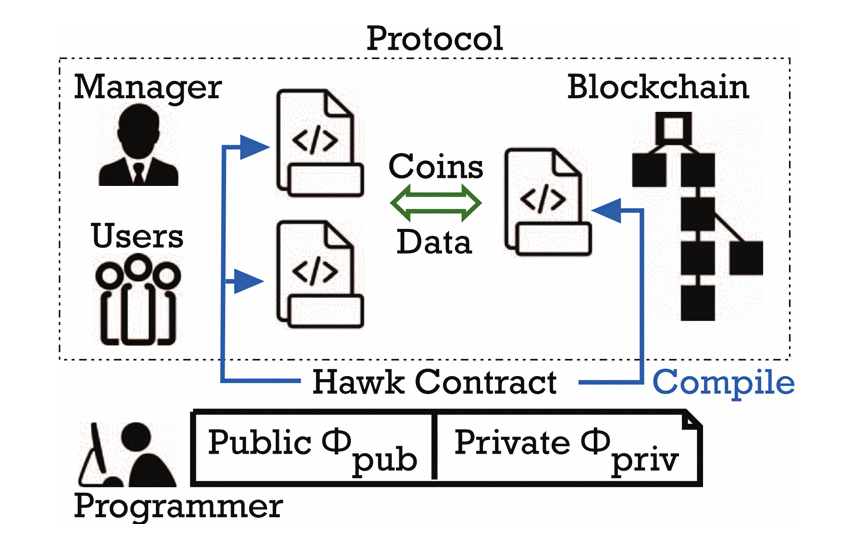
\includegraphics[width=.8\linewidth]{1}
    \caption{Hawk Overview}
    \label{fig1}
\end{figure}

\begin{enumerate}
    \item 私有部分表示为$\phi _{priv}$,它接收各方的输入数据(例如,“石头、纸、剪刀”游戏中的选择)以及货币单位(例如,拍卖中的出价)。$\phi _{priv}$执行计算以确定各方之间的支付分配。例如,在拍卖中,获胜者的出价归卖方所有,而其他人的出价则被退还。私有 \textbf{Hawk} 程序$\phi _{priv}$旨在保护参与者的数据和货币交换。 
    \item 公有部分表示为$\varphi  _{priv}$,$\varphi  _{priv}$不涉及私人数据或金钱。
\end{enumerate}

我们的编译器会将 \textbf{Hawk} 程序编译成以下部分,这些部分共同定义了用户、管理器和区块链之间的加密协议:

\begin{itemize}
    \item 由所有共识节点执行的区块链程序;
    \item 由用户执行的程序;
    \item 由称为经理的特殊促进方执行的程序。(稍后将对其进行解释。)
\end{itemize}

\subsection{安全保障}

\textbf{Hawk} 的安全保障包括两个方面:

\begin{itemize}
    \item \textit{链上隐私}。链上隐私规定,交易隐私是针对公众(即,针对任何未参与合同的一方)提供的——除非合同方自己自愿披露信息。尽管在 \textbf{Hawk} 协议中,用户与区块链交换数据,并依靠它来确保公平性以防止中止,但在私有 \textbf{Hawk} 程序 $\phi _{priv}$ 中交易的资金流和金额以加密方式隐藏在公众的视野之外。非正式地,这是通过向区块链发送“加密”信息,并依靠零知识证明来强制执行合同的正确性和资金节约来实现的。
    \item \textit{合同保障}。虽然链上隐私保护合同方的隐私不受公众(即未参与金融合同的各方)的影响,但合同安全性保护同一合同协议中的各方相互之间。 \textbf{Hawk} 假设合同各方自私地行动以最大化他们自己的经济利益。特别是,它们可以任意偏离规定的协议,甚至提前中止。因此,合同安全是一个多方面的概念,不仅包括机密性和真实性的密码概念,还包括存在作弊和中止行为时的财务公平性。理解合同安全的最好方法是通过一个具体的例子。
\end{itemize}


% 参考文献
\begin{thebibliography}{99}  
    \bibitem{ref1} [online] Available: http://koinify.com.
    \bibitem{ref2} Amazon ec2 pricing, [online] Available: http://aws.amazon.com/ec2/pricing/.
    \bibitem{ref3} Augur, [online] Available: http://www.augur.net/.
    \bibitem{ref4} bitoinj, [online] Available: https://bitcoinj.github.io/.
    \bibitem{ref5} "The rise and rise of bitcoin", Documentary.
    \bibitem{ref6} Skuchain, [online] Available: http://www.skuchain.com/.
    \bibitem{ref7} M. Andrychowicz, S. Dziembowski, D. Malinowski and L. Mazurek, "Secure Multiparty Computations on Bitcoin", S\&P, 2013.
    \bibitem{ref8} G. Asharov, A. Beimel, N. Makriyannis and E. Omri, "Complete characterization of fairness in secure two-party computation of boolean functions", TCC, 2015.
    \bibitem{ref9} M. Bagnoli and B. L. Lipman, "Provision of public goods: Fully implementing the core through private contributions", The Review of Economic Studies, 1989.
    \bibitem{ref10} R. Beaulieu, D. Shors, J. Smith, S. Treatman-Clark, B. Weeks and L. Wingers, The simon and speck families of lightweight block ciphers, [online] Available: http://ia.cr/2013/404.
    \bibitem{ref11} E. Ben-Sasson, A. Chiesa, C. Garman, M. Green, I. Miers, E. Tromer, et al., "Zerocash: Decentralized anonymous payments from Bitcoin", S\&P, 2014.
    \bibitem{ref12} E. Ben-Sasson, A. Chiesa, D. Genkin, E. Tromer and M. Virza, "Snarks for C: verifying program executions succinctly and in zero knowledge", CRYPTO, 2013.
    \bibitem{ref13} E. Ben-Sasson, A. Chiesa, M. Green, E. Tromer and M. Virza, "Secure sampling of public parameters for succinct zero knowledge proofs", S\&P, 2015.
    \bibitem{ref14} E. Ben-Sasson, A. Chiesa, E. Tromer and M. Virza, "Scalable zero knowledge via cycles of elliptic curves", CRYPTO, 2014.
    \bibitem{ref15} E. Ben-Sasson, A. Chiesa, E. Tromer and M. Virza, "Succinct noninteractive zero knowledge for a von neumann architecture", Security, 2014.
    \bibitem{ref16} E. Ben-Sasson and M. Sudan, "Short pcps with polylog query complexity", SIAM J. Comput., 2008.
    \bibitem{ref17} I. Bentov and R. Kumaresan, "How to Use Bitcoin to Design Fair Protocols", CRYPTO, 2014.
    \bibitem{ref18} N. Bitansky, R. Canetti, A. Chiesa and E. Tromer, "Recursive composition and bootstrapping for snarks and proof-carrying data", STOC, 2013.
    \bibitem{ref19} D. Bogdanov, S. Laur and J. Willemson, "Sharemind: A Framework for Fast Privacy-Preserving Computations", ESORICS, 2008.
    \bibitem{ref20} J. Bonneau, A. Miller, J. Clark, A. Narayanan, J. A. Kroll and E. W. Felten, "Research Perspectives and Challenges for Bitcoin and Cryptocurrencies", S\&P, 2015.
    \bibitem{ref21} R. Canetti, "Universally composable security: A new paradigm for cryptographic protocols", FOCS, 2001.
    \bibitem{ref22} R. Canetti, "Universally composable signature certification and authentication", CSF, 2004.
    \bibitem{ref23} R. Canetti, Y. Dodis, R. Pass and S. Walfish, "Universally composable security with global setup", TCC, 2007.
    \bibitem{ref24} R. Cleve, "Limits on the security of coin flips when half the processors are faulty", STOC, 1986.
    \bibitem{ref25} C. Costello, C. Fournet, J. Howell, M. Kohlweiss, B. Kreuter, M. Naehrig, et al., "Geppetto: Versatile verifiable computation", S \& P, 2015.
    \bibitem{ref26} G. Danezis, C. Fournet, M. Kohlweiss and B. Parno, "Pinocchio Coin: building Zerocoin from a succinct pairing-based proof system", PETShop, 2013.
    \bibitem{ref27} C. Decker and R. Wattenhofer, "Bitcoin transaction malleability and mtgox" in ESORICS, Springer, 2014.
    \bibitem{ref28} A. K. R. Dermody and O. Slama, Counterparty announcement, [online] Available: https://bitcointalk.org/index.php?topic=395761.0.
    \bibitem{ref29} I. Eyal and E. G. Sirer, "Majority is not enough: Bitcoin mining is vulnerable", FC, 2014.
    \bibitem{ref30} C. Fournet, M. Kohlweiss, G. Danezis and Z. Luo, "Zql: A compiler for privacy-preserving data processing", USENIX Security, 2013.
    \bibitem{ref31} M. Fredrikson and B. Livshits, "Zø: An optimizing distributing zero-knowledge compiler", USENIX Security, 2014.
    \bibitem{ref32} J. A. Garay, A. Kiayias and N. Leonardos, "The bitcoin backbone protocol: Analysis and applications", Eurocrypt, 2015.
    \bibitem{ref33} R. Gennaro, C. Gentry, B. Parno and M. Raykova, "Quadratic span programs and succinct NIZKs without PCPs", Eurocrypt, 2013.
    \bibitem{ref34} E. Heilman, A. Kendler, A. Zohar and S. Goldberg, "Eclipse attacks on bitcoin's peer-to-peer network", USENIX Security, 2015.
    \bibitem{ref35} A. Juels, A. Kosba and E. Shi, "The ring of gyges: Using smart contracts for crime", Manuscript, 2015.
    \bibitem{ref36} A. Kiayias, H.-S. Zhou and V. Zikas, Fair and robust multi-party computation using a global transaction ledger, [online] Available: http://ia.cr/2015/574.
    \bibitem{ref37} A. Kosba, A. Miller, E. Shi, Z. Wen and C. Papamanthou, Hawk: The blockchain model of cryptography and privacy-preserving smart contracts, [online] Available: http://ia.cr/2015/675.
    \bibitem{ref38} A. Kosba, Z. Zhao, A. Miller, H. Chan, C. Papamanthou, R. Pass, et al., How to use snarks in universally composable protocols, 2015, [online] Available: https://eprint.iacr.org/2015/1093.
    \bibitem{ref39} B. Kreuter, B. Mood, A. Shelat and K. Butler, "PCF: A portable circuit format for scalable two-party secure computation", Security, 2013.
    \bibitem{ref40} R. Kumaresan and I. Bentov, "How to Use Bitcoin to Incentivize Correct Computations", CCS, 2014.
    \bibitem{ref41} C. Liu, X. S. Wang, K. Nayak, Y. Huang and E. Shi, "ObliVM: A programming framework for secure computation", S\&P, 2015.
    \bibitem{ref42} S. Meiklejohn, M. Pomarole, G. Jordan, K. Levchenko, D. McCoy, G. M. Voelker, et al., "A fistful of bitcoins: characterizing payments among men with no names", IMC, 2013.
    \bibitem{ref43} I. Miers, C. Garman, M. Green and A. D. Rubin, "Zerocoin: Anonymous Distributed E-Cash from Bitcoin", S\&P, 2013.
    \bibitem{ref44} A. Miller, M. Hicks, J. Katz and E. Shi, "Authenticated data structures generically", POPL, 2014.
    \bibitem{ref45} A. Miller and J. J. LaViola, "Anonymous Byzantine Consensus from Moderately-Hard Puzzles: A Model for Bitcoin", 2014.
    \bibitem{ref46} M. S. Miller, C. Morningstar and B. Frantz, "Capability-based financial instruments", FC, 2001.
    \bibitem{ref47} N. Mouha, B. Mennink, A. Van, D. Watanabe, B. Preneel and I. Verbauwhede, "Chaskey: An efficient mac algorithm for 32-bit microcontrollers" in Selected Areas in Cryptography-SAC 2014, Springer, pp. 306-323, 2014.
    \bibitem{ref48} S. Nakamoto, Bitcoin: A Peer-to-Peer Electronic Cash System, 2009, [online] Available: http://bitcoin.org/bitcoin.pdf.
    \bibitem{ref49} B. Parno, C. Gentry, J. Howell and M. Raykova, "Pinocchio: Nearly practical verifiable computation", S\&P, 2013.
    \bibitem{ref50} R. Pass and Abhi Shelat, "Micropayments for peer-to-peer currencies", CCS, 2015.
    \bibitem{ref51} A. Rastogi, M. A. Hammer and M. Hicks, "Wysteria: A programming language for generic mixed-mode multiparty computations", S\&P, 2014.
    \bibitem{ref52} D. Ron and A. Shamir, "Quantitative Analysis of the Full Bitcoin Transaction Graph", FC, 2013.
    \bibitem{ref53} N. Szabo, "Formalizing and securing relationships on public networks", 1997.
    \bibitem{ref54} N. van Saberhagen, Cryptonote v 2.0, 2013, [online] Available: https://goo.gl/kfojVZ.
    \bibitem{ref55} W. Vickrey, "Counterspeculation auctions and competitive sealed tenders", Journal of finance, 1961.
    \bibitem{ref56} R. S. Wahby, S. T. V. Setty, Z. Ren, A. J. Blumberg and M. Walfish, "Efficient RAM and control flow in verifiable outsourced computation", NDSS, 2015.
    \bibitem{ref57} G. Wood, Ethereum: A secure decentralized transaction ledger, [online] Available: http://gavwood.com/paper.pdf.
    \bibitem{ref58} L. Zheng, S. Chong, A. C. Myers and S. Zdancewic, "Using replication and partitioning to build secure distributed systems", S\&P, 2003.
    \bibitem{ref59} G. Zyskind, O. Nathan and A. Pentland, Enigma: Decentralized computation platform with guaranteed privacy.
\end{thebibliography}
\backmatter
\end{document}